%\documentclass[notitlepage,aps,prd,twocolumn,nofootinbib]{revtex4-1}
\documentclass[notitlepage,aps,prd,nofootinbib]{revtex4-1}

\usepackage{subfig}
%\usepackage[colorinlistoftodos]{todonotes}
\usepackage{float}

%\usepackage[protrusion=true,expansion=true]{microtype}
\usepackage{amsmath}
\usepackage{amssymb}
\usepackage{bbm}
\usepackage{ulem}
%\usepackage{feynmp-auto}
%\usepackage{slashed}
%\usepackage[absolute,overlay]{textpos}
\usepackage[usenames, dvipsnames]{color}
\usepackage{graphicx}
\usepackage{listings}
\usepackage{epsfig}
\usepackage{hyperref}
%\usepackage{tikz}
\usepackage{enumerate}
%\usepackage{fixltx2e} % buggy
\usepackage[compatibility=false]{caption}
%\usepackage{subcaption} % doesn't work with subfigure
\usepackage{pdfpages}
%\usepackage{setspace}
\usepackage{verbatim}

\DeclareRobustCommand{\orderof}{\ensuremath{\mathcal{O}}}

\definecolor{dukeblue}{RGB}{0,0,156}
\definecolor{dukedarkblue}{RGB}{0,26,87}
\definecolor{dukeblack}{RGB}{79,79,79}
\definecolor{dukegray}{RGB}{79,79,79}
\definecolor{dukesecbrown}{RGB}{217,200,158}
\definecolor{dukesecblue}{RGB}{127,169,174}

%\renewcommand*{\thefootnote}{\fnsymbol{footnote}}

%%%%%%%%%%%%%%%%%%%%%%%%%%%%%%%%%%%%%%%%%%%%%%%%%%%%%%%%%%%%%%%%%%%%%%%%%%%%%%%%%%%%%
\hypersetup{
    breaklinks,
    baseurl       = http://,
    pdfborder     = 0 0 0,
    pdfpagemode   = UseNone,% do not show thumbnails or bookmarks on opening
    pdfstartpage  = 1,
    bookmarksopen = true,
    bookmarksdepth= 2,% to show sections and subsections
% revtex needs author and title declared after \begin{document}, so have to hard code them...
%    pdfauthor     = {\@author},
%    pdftitle      = {\@title},
    pdfauthor     = {Matthew Epland},
    pdftitle      = {Phys 566 HW3},
    pdfsubject    = {},
    pdfkeywords   = {}}


% Code import settings
%%%%%%%%%%%%%%%%%%%%%%%%%%%%%%%%%%%%%%%%%%%%%%%%%%%%%%%%%%%%%%%%%%%%%%%%%%%%%%%%%%%%%
\definecolor{mygreen}{rgb}{0,0.6,0}
\definecolor{mygray}{rgb}{0.5,0.5,0.5}
\definecolor{mymauve}{rgb}{0.58,0,0.82}

%\lstset{ %
\lstdefinestyle{python}{ %
  backgroundcolor=\color{white},   % choose the background color; you must add \usepackage{color} or \usepackage{xcolor}
  basicstyle=\scriptsize,          % the size of the fonts that are used for the code
  breakatwhitespace=false,         % sets if automatic breaks should only happen at whitespace
  breaklines=true,                 % sets automatic line breaking
  captionpos=b,                    % sets the caption-position to bottom
  commentstyle=\color{mygreen},    % comment style
  deletekeywords={...},            % if you want to delete keywords from the given language
  escapeinside={\%*}{*)},          % if you want to add LaTeX within your code
  extendedchars=true,              % lets you use non-ASCII characters; for 8-bits encodings only, does not work with UTF-8
  frame=single,	                   % adds a frame around the code
  keepspaces=true,                 % keeps spaces in text, useful for keeping indentation of code (possibly needs columns=flexible)
  keywordstyle=\color{blue},       % keyword style
  language=Python,                 % the language of the code
  otherkeywords={*,...},           % if you want to add more keywords to the set
  numbers=left,                    % where to put the line-numbers; possible values are (none, left, right)
  numbersep=5pt,                   % how far the line-numbers are from the code
  numberstyle=\tiny\color{mygray}, % the style that is used for the line-numbers
  rulecolor=\color{black},         % if not set, the frame-color may be changed on line-breaks within not-black text (e.g. comments (green here))
  showspaces=false,                % show spaces everywhere adding particular underscores; it overrides 'showstringspaces'
  showstringspaces=false,          % underline spaces within strings only
  showtabs=false,                  % show tabs within strings adding particular underscores
  stepnumber=5,                    % the step between two line-numbers. If it's 1, each line will be numbered
  stringstyle=\color{mymauve},     % string literal style
  tabsize=2,	                   % sets default tabsize to 2 spaces
%  title=\lstname                   % show the filename of files included with \lstinputlisting; also try caption instead of title
  title={\protect\filename@parse{\lstname}\protect\filename@base.\filename@ext},
  firstnumber=0,
%  linewidth=0.95\textwidth
  xleftmargin=0.01\textwidth,
  xrightmargin=0.01\textwidth
}

\lstdefinestyle{output}{ %
  backgroundcolor=\color{white},   % choose the background color; you must add \usepackage{color} or \usepackage{xcolor}
  basicstyle=\scriptsize,          % the size of the fonts that are used for the code
  breakatwhitespace=false,         % sets if automatic breaks should only happen at whitespace
  breaklines=true,                 % sets automatic line breaking
  captionpos=b,                    % sets the caption-position to bottom
  escapeinside={\%*}{*)},          % if you want to add LaTeX within your code
  frame=single,	                   % adds a frame around the code
  keepspaces=true,                 % keeps spaces in text, useful for keeping indentation of code (possibly needs columns=flexible)
  numbers=left,                    % where to put the line-numbers; possible values are (none, left, right)
  numbersep=5pt,                   % how far the line-numbers are from the code
  numberstyle=\tiny\color{mygray}, % the style that is used for the line-numbers
  rulecolor=\color{black},         % if not set, the frame-color may be changed on line-breaks within not-black text (e.g. comments (green here))
  stepnumber=5,                    % the step between two line-numbers. If it's 1, each line will be numbered
  tabsize=2,	                   % sets default tabsize to 2 spaces
%  title=\lstname                   % show the filename of files included with \lstinputlisting; also try caption instead of title
  title={\protect\filename@parse{\lstname}\protect\filename@base.\filename@ext},
  firstnumber=0,
%  linewidth=0.95\textwidth
  xleftmargin=0.01\textwidth,
  xrightmargin=0.01\textwidth
}


%%%%%%%%%%%%%%%%%%%%%%%%%%%%%%%%%%%%%%%%%%%%%%%%%%%%%%%%%%%%%%%%%%%%%%%%%%%%%%%%%%%%%
\begin{document}

\title{PHYS 566 HW3}
\author{Matthew Epland}
\affiliation{Department of Physics, Duke University, Durham, NC 27707, USA}
%\institute{Duke University}

\date{\today}

\begin{abstract}
TODO
\end{abstract}\maketitle


\section{Introduction}
\label{sec:intro}
TODO

\section{Theory}
\label{sec:theory}
We can numerically model an objects trajectory by splitting up Newton's 2nd Law (\ref{eq:newton2}) into coupled first order differential equations (\ref{eq:deqs}) that we can apply the Euler method (\ref{eq:euler1}) to.

\begin{equation} \label{eq:newton2}
m \frac{d^2 \mathbf{r}}{d t^2} = \mathbf{F}_{\text{net}} 
\end{equation}

\begin{equation} \label{eq:deqs}
\frac{d \mathbf{v}}{d t} = \frac{1}{m} \mathbf{F}_{\text{net}}
\qquad
\frac{d \mathbf{r}}{d t} = \mathbf{v}
\end{equation}

\begin{equation} \label{eq:euler1}
\mathbf{r}\left(t + \Delta t\right) \approx \mathbf{r}\left(t\right) + \frac{d \mathbf{r}}{d t} \Delta t = \mathbf{r}\left(t\right) + \mathbf{v}\left(t\right) \Delta t
\qquad
\mathbf{v}\left(t + \Delta t\right) \approx \mathbf{v}\left(t\right) + \frac{d \mathbf{v}}{d t} \Delta t = \mathbf{v}\left(t\right) + \frac{1}{m}\mathbf{F}_{\text{net}}\left(t\right) \Delta t
\end{equation}

These equations are the heart of our model. All we need do now is split the vectors up into $\hat{\mathbf{x}}$ and $\hat{\mathbf{y}}$ components, using some simple trigonometry when necessary (\ref{eq:theta}), and set the initial conditions (\ref{eq:initial_conditions}).

\begin{equation} \label{eq:theta}
\theta\left(t\right) = \arctan\left(\frac{v_{y}(t)}{v_{x}(t)}\right)
\qquad
\mathbf{v}\left(t\right) = \big|\mathbf{v}\left(t\right)\big|
\begin{pmatrix}
  \cos(\theta) \\
  \sin(\theta)
\end{pmatrix}
\end{equation}

\begin{equation} \label{eq:initial_conditions}
\mathbf{r}\left(0\right) = 
\begin{pmatrix}
  0 \\
  0
\end{pmatrix}
\qquad
\mathbf{v}\left(0\right) = v_{0}
\begin{pmatrix}
  \cos(\theta_{0}) \\
  \sin(\theta_{0})
\end{pmatrix}
\end{equation}


In this assignment we are considering gravity as well as drag forces in four different cases:

\subsection{Ideal} \label{subsec:ideal}
Without drag we have the simplest $\mathbf{F}_{\text{net}}$ (\ref{eq:F_ideal}).

\begin{equation} \label{eq:F_ideal}
\mathbf{F}_{\text{net}} = -m g\hat{\mathbf{y}}
\end{equation}

\subsection{Smooth Ball with Drag} \label{subsec:smooth_drag}
Adding $\mathbf{F}_{\text{drag}} = - C \rho A \big|\mathbf{v}\left(t\right)\big|^2 \hat{\mathbf{v}}$, we have (\ref{eq:F_smooth_drag}).

\begin{equation} \label{eq:F_smooth_drag}
\mathbf{F}_{\text{net}} = - C \rho A \big|\mathbf{v}\left(t\right)\big|^2 
\begin{pmatrix}
  \cos(\theta) \\
  \sin(\theta)
\end{pmatrix}
-m g\hat{\mathbf{y}}
\end{equation}

TODO


\section{Results}
\label{sec:results}
TODO

\begin{comment}
\begin{figure}[!htbc]
%\begin{figure}
  \centering
  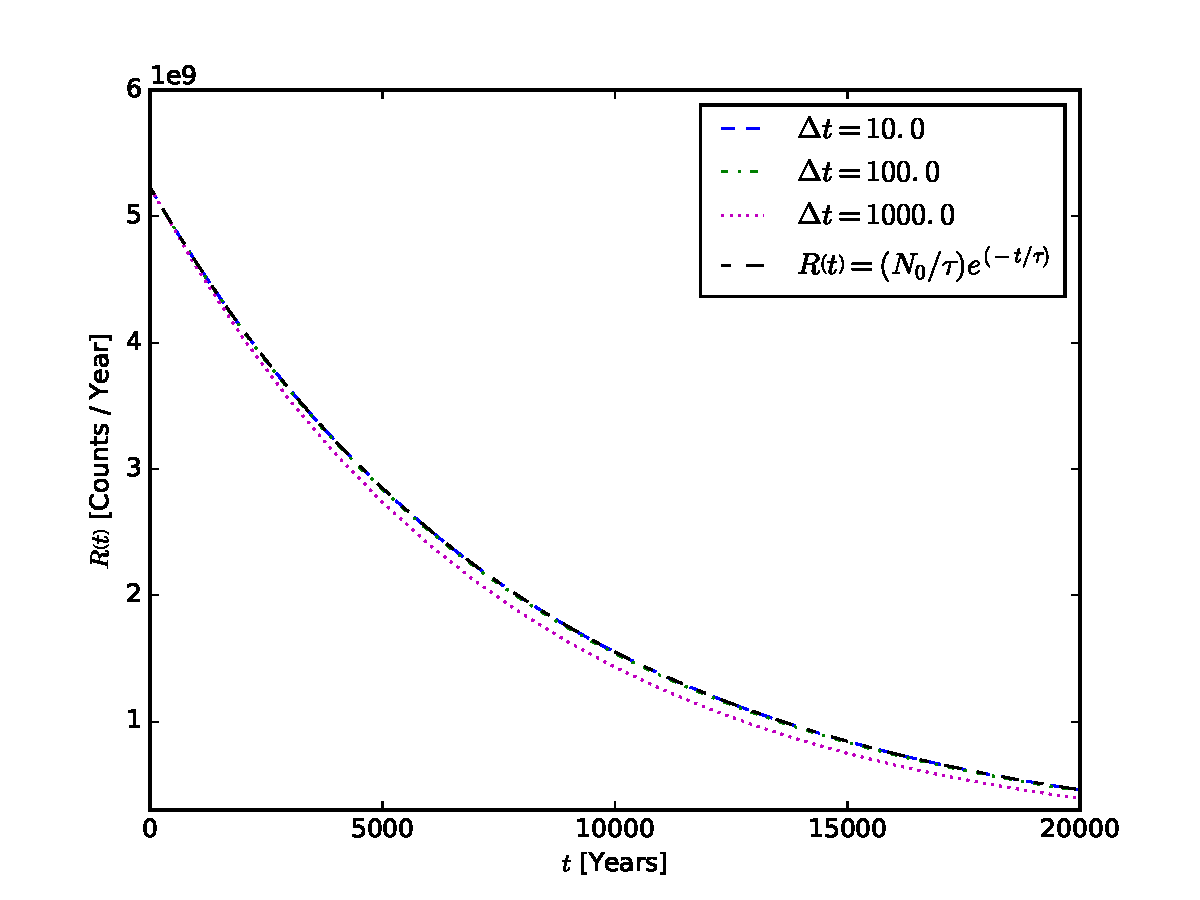
\includegraphics[width=.70\textwidth]{output/plot.pdf}
	{\par\nobreak\rule[9pt]{35em}{0.5pt}\vspace{-5mm}}
	\caption{$R\left(t\right)$ calculated numerically with three different time steps, $\Delta t$, and the exact solution.}
	\label{fig:plot}
\end{figure}

\end{comment}


\section{Conclusions}
\label{sec:Conclusions}
TODO

The Python source code used to produce these results can be found online at \url{http://github.com/mepland/PHYS_566_Computational_HW/tree/master/hw3/code}, and is included in Section~\ref{sec:code}.

\clearpage
\section{Supporting Material}
\label{sec:Supporting_Material}

\clearpage
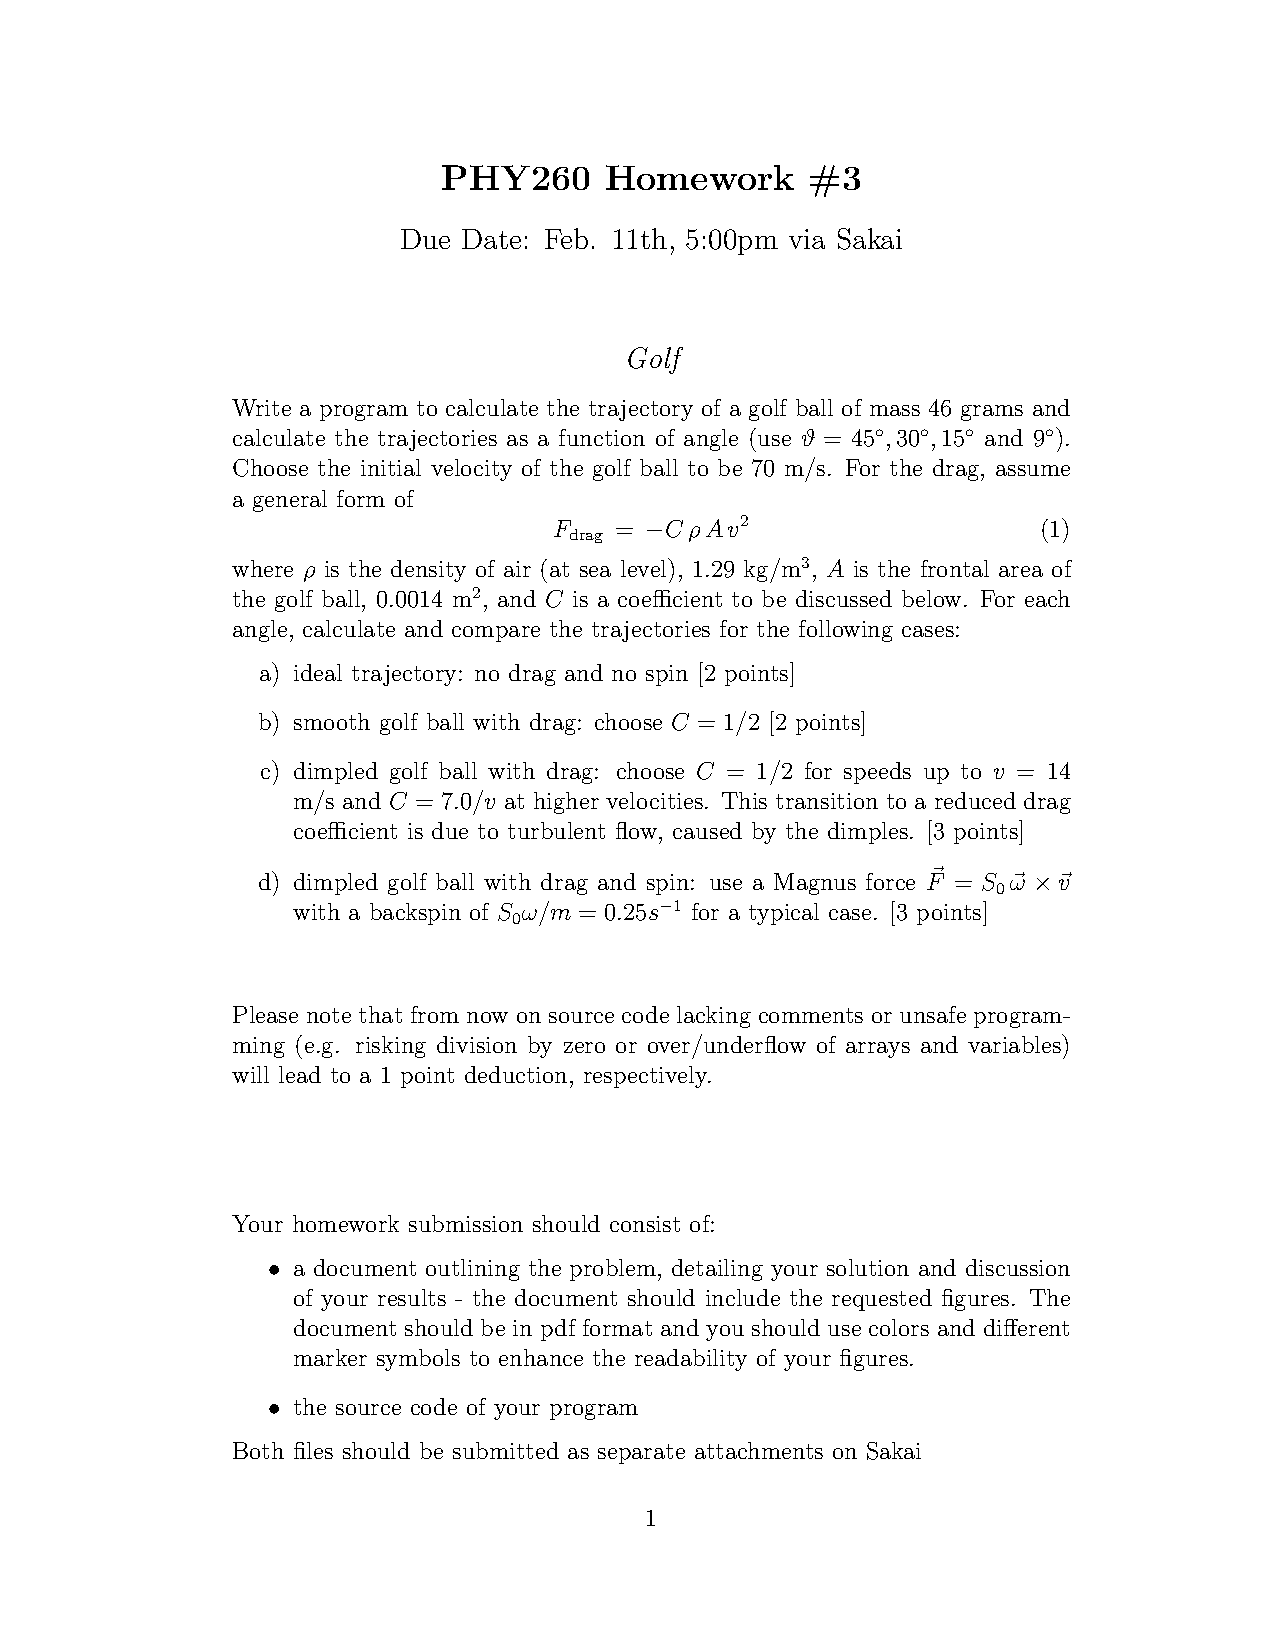
\includepdf{../homework3.pdf}

\clearpage
\section{Code}
\label{sec:code}

\lstinputlisting[style=python]{../code/golf.py}

\end{document} %%% end of doc %%%




\bibliographystyle{bib_files/styles/atlasBibStyleWoTitle}
\bibliography{bib_files/my_bib.bib}


